%%%%%%%%%%%%%%%%%%%%%%%%%%%%%%%%%%%%%
%%%%% PHYS305 Assignment 4
%%%%% Zachary Martin
%%%%% 13 February 2019
%%%%%%%%%%%%%%%%%%%%%%%%%%%%%%%%%%%%%

\documentclass[aps,prl,twocolumn,superscriptaddress]{revtex4-1}

\usepackage{graphicx}  % this is the up-to-date package for all figures
\graphicspath{{pictures/}} 	% Set Graphics Path
\usepackage{siunitx} % Scientific Notation and Units
\usepackage{amsmath, amssymb, gensymb, mathtools, bm, bigints} 	% Mathematical Tools
\usepackage{verbatim}  % for the comment environment
\usepackage{color}
% \usepackage{arydshln} % Dashed lines in table

% For inserting code snippets
\usepackage{listings}
\usepackage{xcolor}
\lstset { %
    language=C++,
    backgroundcolor=\color{black!5}, % set backgroundcolor
    basicstyle=\footnotesize,% basic font setting
}

% Shortcut Commands
\newcommand{\paren}[1]{\left( #1 \right)} 	% Parentheses for complicated expressions
\newcommand{\bparen}[1]{\left[ #1 \right]}	% Bracket parentheses for complicated expressions
\newcommand{\cmod}[1]{\left| #1 \right|}	% Mod or Absolute value

\bibliographystyle{apsrev}

% these are some custom control of the page size and margins
% \topmargin= 0.2in  % these 1st two may be needed for some computers
\textheight=9in
\textwidth=6.5in
% these next two lines give us centered text
\oddsidemargin=0cm
\evensidemargin=0cm

\begin{document}

% Title Contents
\title{PHYS 305 Assignment 4: Analyzing the Behavior of Random Walks.}
\author{Zachary Martin}
\affiliation{University of Hawaii at Manoa}
\date{13 February 2019}

\begin{abstract}
In this assignment, we examine the macro-level behavior of a random walk. To accomplish this, we have written a C++ program to utilize the drand48() function to generate values between zero and one. More specifically, we will analyze how the average distance from the origin after $S$ steps compares to the number of steps taken. The affect of varying the number of trials, $N$, will also be examined. We were able confirm the relation to be a power law of $0.5$. In the process, we also found that precision of the results depend deeply on the number of trials, and slightly on the maximum number of steps. We also discover that the drand48() exhibits a slight bias.
\end{abstract}

\maketitle

\section{Introduction and Overview}
Randomness plays a major role in many physical systems; particle motion, nuclear decay, gene and protein production, and chaotic or turbulent forces to name a few \cite{Laulima}. The study of the randomness of a particular system can lead to significant theories that help to describe and understand how the systems are being affected and how we can extrapolate data from a random system. We can understand this through statistics, examining the probability distributions of these random factors. Fundamental theories in physics are dominated by this kind of study, such as quantum mechanics, statistical mechanics, thermodynamics, and chaos theory.

Thus, we will examine a simple example of random motion, a random walk, and examine the statistical properties we can gain from it. Specifically, we want to see the distribution of the endpoints in the random walks as well as how the average distance compares to the number of steps taken. To do this, we will run a number of trials of random walks for different number of steps and determine how the distance from the starting point (we choose the origin) relates to the number of steps. 


\begin{figure}[htbp]
  	\begin{center}
 		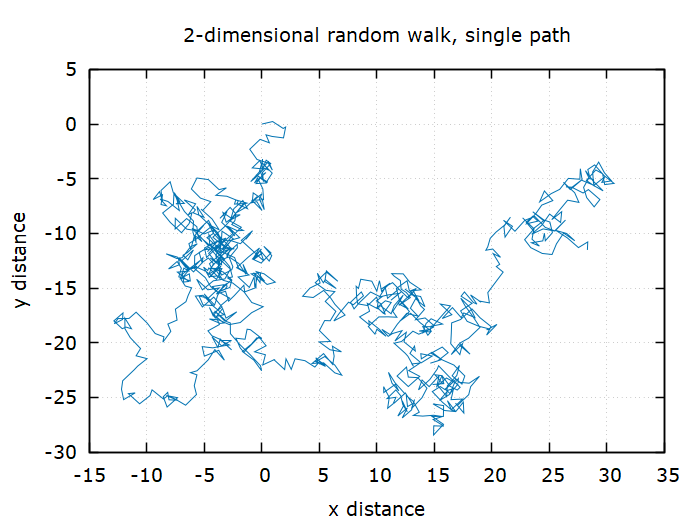
\includegraphics[scale=0.3]{path.png} 
 		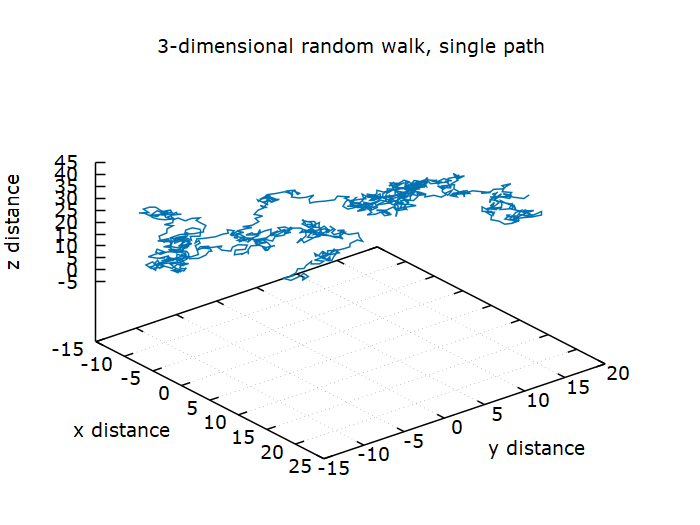
\includegraphics[scale=0.35]{path3d.png}
  		\caption{Random walk paths in the 2D and 3D cases, starting at 0,0. Path selected from one of the 1000 trials.}
  		\label{gr:path}
 	\end{center}
\end{figure}
 
\section{Description of Computational Problem}
The main problem for this experiment is running multiple trials of random walks and computing the step directions and total distance. The role of a computer program is then obvious. We must write a script to not only generate a random walk, but to generate a multitude of them. We start with a 2D random walk, and then move to the 3D case. To simulate randomness, we use the drand48() function in C++ to generate random double values within the range [0.0, 1.0). We can select a range to choose a random value from by simply multiplying the range by the random number generator. We can output the data obtained by creating file streams for the relevant data. We want to list out the average distances, the endpoints for each trial, and choose a single path to trace, that is, listing out the coordinates for every step. 

\section{Relevant Equations}
First, we need to be able to describe how the 'particle' can move randomly in the x and y directions. Simply, we choose a random angle, $\theta$, between $0$ and $2 \pi$ and choose unit step size. Then
\begin{align}
x &= \cos \theta \label{eqn:x2d} \\ 
y &= \sin \theta ~.	\label{eqn:y2d}
\end{align}
Now we allow this to continue, adding to the previous the same expressions in Equations \ref{eqn:x2d} and \ref{eqn:y2d} for different random angles until a certain number of steps, $S$, have been reached. In each step, we need to calculate the distance, $r$, from the origin. For 2D, this is simply
\begin{equation}
r = \sqrt{x^2 + y^2} ~. \label{eqn:r2d}
\end{equation}
Implemented into the program, we have
\begin{lstlisting}
x=y=0; // Starting point
for (i=1; i<=Nmax; i++){
	x += cos(drand48()*2.*M_PI);
	y += sin(drand48()*2.*M_PI);
	r[i] += sqrt(x*x + y*y);
	}
\end{lstlisting}
This will happen for a given amount of trials, $N$. Then we must average the distances per step from all of the trials. To do this, we use
\begin{equation}
\bar{r}(i) = \frac{1}{N}\paren{\displaystyle \sum_{j}^{N} r(i)_j} ~, \label{eqn:ravg}
\end{equation}
where $r(i)_j$ is the distance from the origin after $i$ steps in the $j$th trial. Statistically, the error in each step is then
\begin{equation}
\delta \bar{r}(i) = \frac{\sqrt{N}}{N} \bar{r}(i) = N^{-3/2} \paren{\displaystyle \sum_{j}^{N} r(i)_j} ~. \label{eqn:ravgerr}
\end{equation}
For the 3D case, we must choose spherical coordinates. So then for unit steps,
\begin{align}
x &= \sin \phi \cos \theta \label{eqn:x3d} \\
y &= \sin \phi \sin \theta \label{eqn:y3d} \\
z &= \cos \phi ~. \label{eqn:z3d}
\end{align}
Note that the volume element 
\begin{equation}
d \Omega = \sin \phi d\theta d\phi
\end{equation}
is a function of $\phi$. Thus we cannot just choose the angles randomly between $0$ to $2 \pi$ and $0$ to $\pi$ if we want a truly random distribution. Instead, we use
\begin{align}
\theta &= u 2 \pi \label{eqn:thetarand} \\
\phi &= \cos^{-1} \paren{2 v - 1} ~, \label{eqn:phirand}
\end{align}
where $u, v$ are random points in the range [0.0, 1.0) \cite{3drand}. Now the distance from the origin is
\begin{equation}
r = \sqrt{x^2 + y^2 + z^2} ~.
\end{equation}
Implementing this into the program, we have
\begin{lstlisting}
x=y=z=0;	// starting point  
for (i=1; i<=Nmax; i++){
	theta = 2.*M_PI*drand48();
	phi = acos(2.*drand48() - 1.);
	x += sin(phi)*cos(theta);
	y += sin(phi)*sin(theta);
	z += cos(phi);
	r[i] += sqrt(x*x + y*y + z*z);
	}
\end{lstlisting}
The expressions for average distance per step per trial and the error stays the same, so Equations \ref{eqn:ravg} and \ref{eqn:ravgerr} hold.
When we examine the average distance per step, we should expect to find a curve of the form
\begin{equation}
\bar{r}(i) = i^p ~. \label{eqn:fit}
\end{equation}
Statistically, we expect the parameter $p$ to be $p = 0.5$.

\section{Results and Graphs}

\begin{table}[h] % table environment to enable captions and labels, [h] = 'here'
	\begin{center}
		\begin{tabular*}{\columnwidth}{| c c  @{\extracolsep{\fill}} c c c | }
		\hline
 		$N$ & $S$ & $p$ & $\delta p ~(10^{-5})$ & Diff (\%) \\
 		\hline\hline
 		$1000$ & $1000$ & $0.4815$ & $4.068$ & $3.7$ \\
 		$1000$ & $10000$ & $0.4859$ & $1.19$ & $2.8$ \\
 		$10$ & $10000$ & $0.5094$ & $8.456$ & $1.9$ \\
 		$10$ & $100000$ & $0.5091$ & $2.047$ & $1.8$ \\
 		$4$ & $1000$ & $0.5048$ & $64.05$ & $0.96$ \\
 		*$1000$ & $10000$ & $0.4903$ & $1.37$ & $1.94$ \\
 		\hline
		\end{tabular*}
	\caption{Different parameters $p$ from the fits in Figure \ref{gr:fit} using Equation \ref{eqn:fit}. $N$ is the number of trials and $S$ is the number of steps. These were fitted using Gnuplot. *This is the result for the 3D case.} \label{tbl:p}
	\end{center}
\end{table}

\begin{figure}[htbp]
  	\begin{center}
 		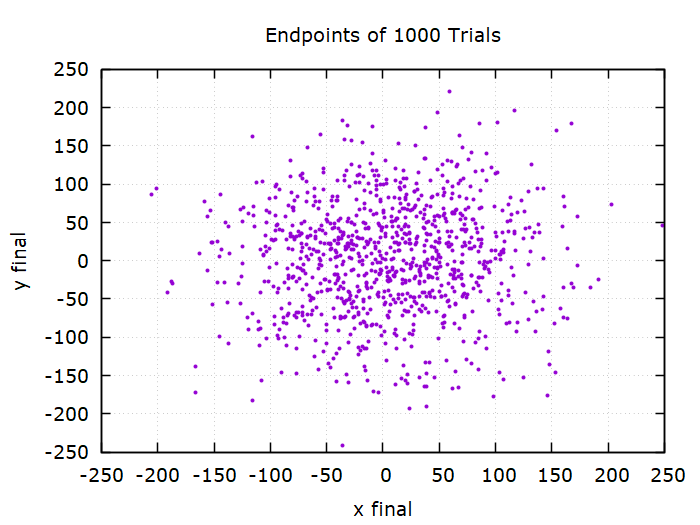
\includegraphics[scale=0.3]{endpt.png} 
 		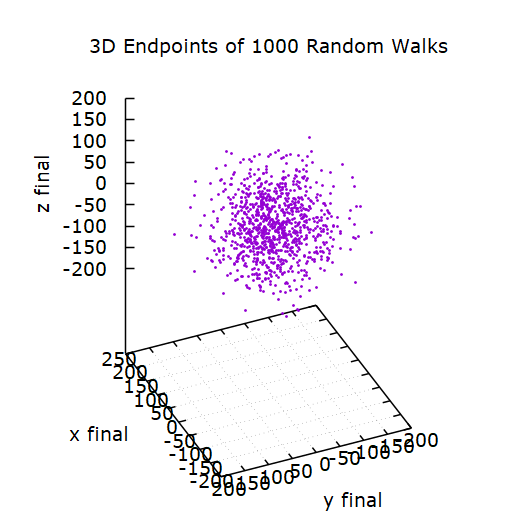
\includegraphics[scale=0.5]{endpt3d.png}
  		\caption{A scatter plot of the endpoints of the paths for 1000 trials in both the 2D and 3D case. Note that the axes are not equally spaced in the 2D case; the distribution should look circular. In the 3D case, we can see clearly a spherical distribution.}
  		\label{gr:endpt}
 	\end{center}
\end{figure}

\begin{figure}[htbp]
  	\begin{center}
 		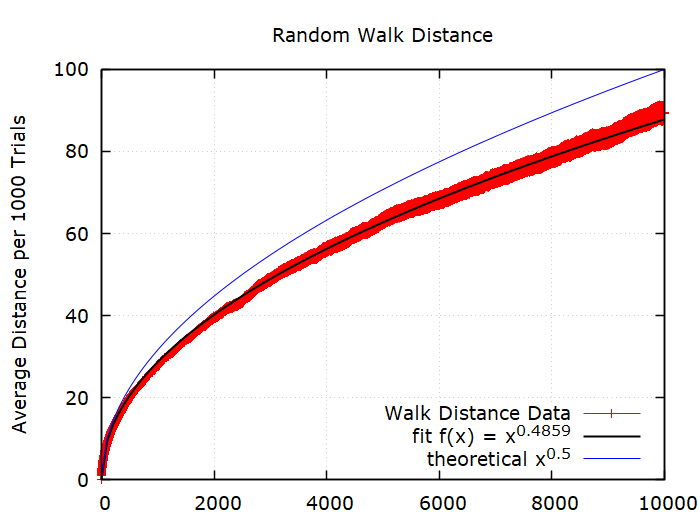
\includegraphics[scale=0.28]{fit.png} 
 		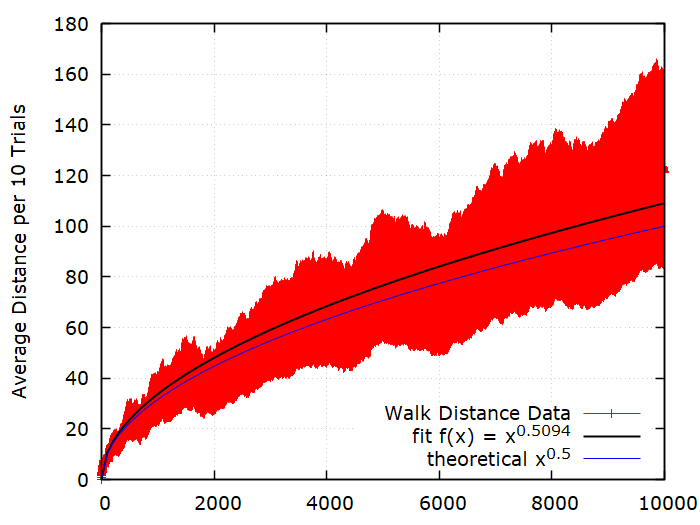
\includegraphics[scale=0.28]{fit1010000.png}
 		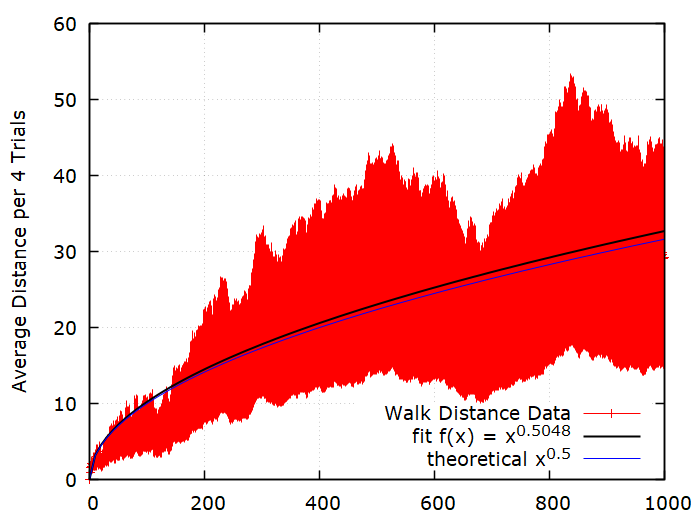
\includegraphics[scale=0.28]{fit41000.png}
 		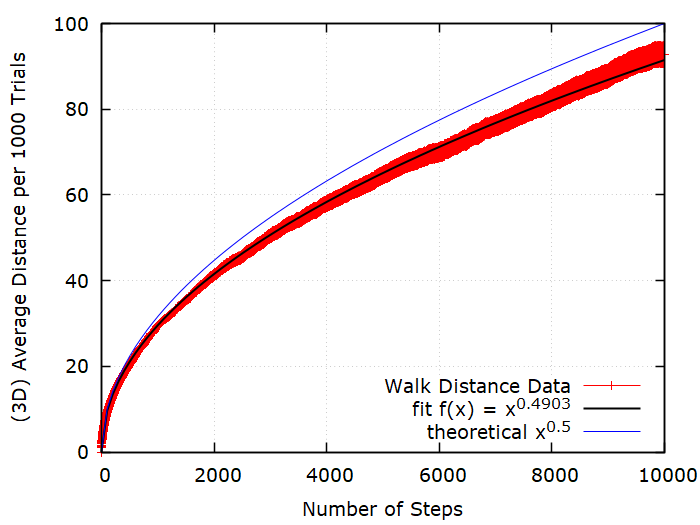
\includegraphics[scale=0.28]{fit3d.png}
  		\caption{The average distance vs steps for different number of maximum steps and trials. The fits for each show a very close agreement to the theoretical. Note that the width of the points indicates the error bar.}
  		\label{gr:fit}
 	\end{center}
\end{figure}

\section{Discussion and Analysis}
First, we can notice that the endpoints for each trial in Figure \ref{gr:endpt} show uniform distributions in all directions. This is exactly what we expect for a random distribution. We can recognize each distribution in a given direction to be a Gaussian distribution. 
Now, we can examine the behavior of the average distance as a function of the number of steps from Figure \ref{gr:fit} and Table \ref{tbl:p}. We notice immediately the affect of changing the number of trials. For $N = 4, 10$, the errors are incredibly large. From Equation \ref{eqn:ravgerr}, we can see that the errors are proportional to $N^{-3/2}$ and so having a smaller number of trials will clearly give greater errors than larger numbers of trials. However, we found that a smaller number of trials led to a smaller percent difference. But also notice that the error increased by a whole magnitude. We can also notice that a smaller number of steps also leads to an increase in error, as well as an increase in percent difference. But the affect of changing the number steps is not as significant as changing the number of trials. From each run-through, we can see that the best was the 3D case for $N = 1000$ and $S = 10000$. Another trend we can notice is that at large numbers of trials, the data comes up short of the theoretical curve whereas the low trial number results are over the theoretical curve.

\section{Conclusions}
We were able to create a C++ program to simulate numerous random walks and average over them to determine the overall behavior of the ending distance to the origin. We found that a large number of trials and steps works best to find precise results. We confirmed the theoretical power law that describes the nature of the distance as a function of steps.
The slight bias mentioned earlier could be a result of the random number generator that we used in the program. The random number generators are not perfectly random. They are based on algorithms based on a given seed. But some are able to simulate randomness better than others. It may be worth it to repeat this experiment with different random number generators and compare the results then.
It is evident that despite the random nature of a physical system, there are still macro-level aspects that we can analyze to help us understand and numerically predict things about the system. We have found that in dealing with these random systems, we require a large number of trials to gain a precise behavior. This is why the use of computational methods are significant in physics. 

\section*{Acknowledgments}
\setlength{\parindent}{0cm}

\bibliographystyle{aipauth4-1}
\bibliography{bib4}



\end{document}